%% fig05-two-pass-error, caption is in docs/figures/README.md
\documentclass[border=8pt]{standalone}
% Shared preamble for the interpolation-geometry figures.
% \input by every figNN-*.tex. 
\usepackage[T1]{fontenc}
\usepackage{amsmath,amssymb}
\usepackage{tikz}
\usetikzlibrary{shapes.misc,arrows.meta,calc,decorations.pathreplacing,positioning,fit,backgrounds}

\definecolor{ink}{HTML}{1A1A1A}
\definecolor{gridc}{HTML}{9AA3AD}
\definecolor{accent}{HTML}{1F5FA9}
\definecolor{good}{HTML}{2E7D4F}
\definecolor{bad}{HTML}{B03030}
\definecolor{soft}{HTML}{E6EDF7}
\definecolor{softg}{HTML}{E3F0E8}
\definecolor{softr}{HTML}{F8E6E6}
\definecolor{amber}{HTML}{B8860B}


\tikzset{
  gpt/.style={circle,fill=ink,inner sep=1.15pt},
  ghost/.style={circle,draw=gridc,fill=white,inner sep=1.15pt},
  dep/.style={cross out,draw=accent,thick,inner sep=1.6pt,minimum size=4pt},
  traj/.style={gridc,dotted,thick,-{Stealth[length=2mm]}},
  htraj/.style={accent,very thick,-{Stealth[length=2.6mm]}},
  lbl/.style={font=\footnotesize},
  slbl/.style={font=\scriptsize},
}

\begin{document}
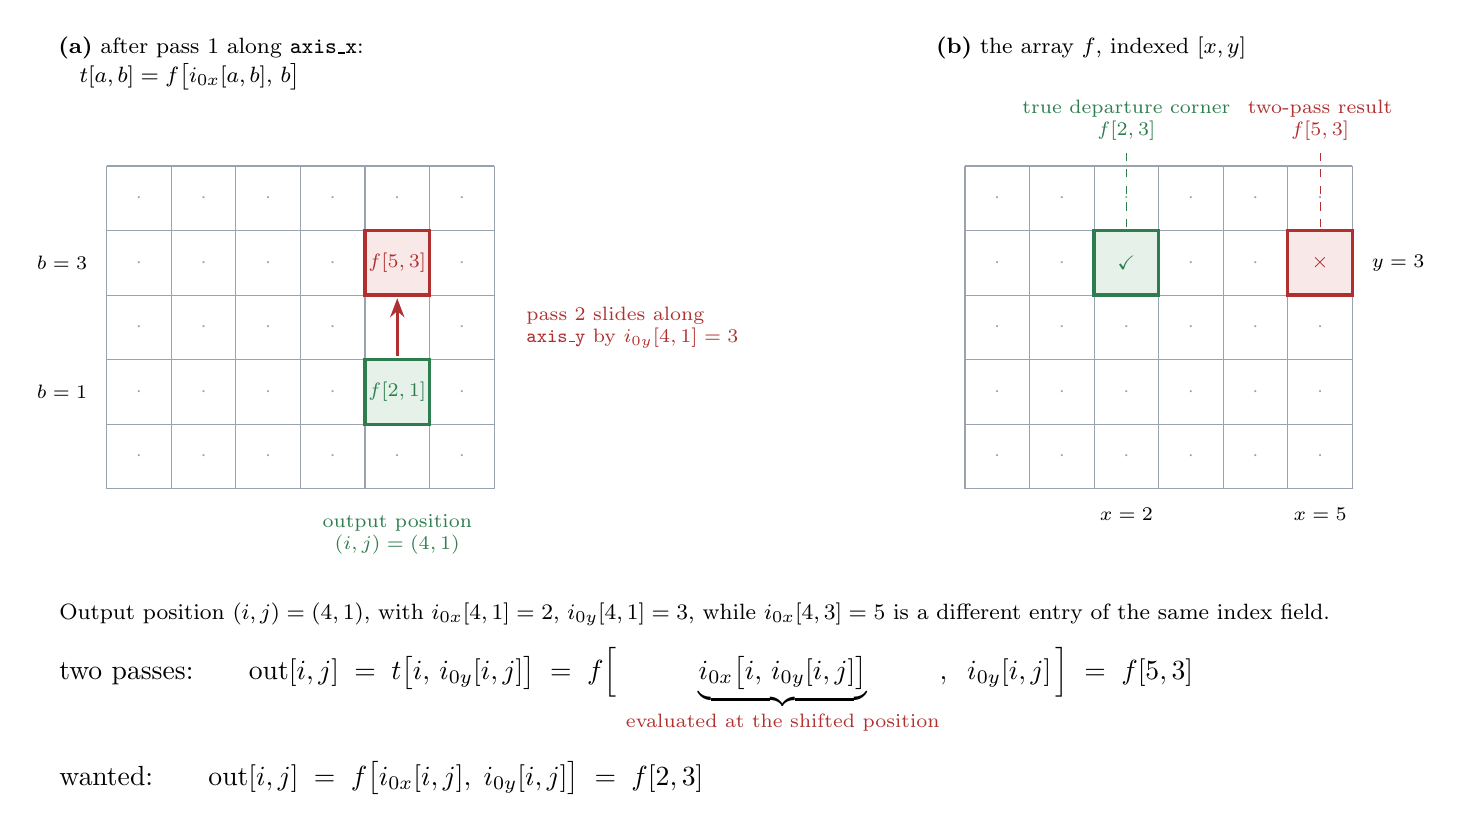
\begin{tikzpicture}[x=0.82cm,y=0.82cm]
  % ---------- intermediate array t ----------
  \begin{scope}
    \node[lbl,anchor=north west,align=left] at (-0.9,7.15)
      {\textbf{(a)} after pass 1 along \texttt{axis\_x}:\\[1pt]
       \hspace{0.9em}$t[a,b]=f\big[i_{0x}[a,b],\,b\big]$};
    \draw[gridc,thin] (0,0) grid[step=1] (6,5);
    \foreach \i in {0,...,5} \foreach \j in {0,...,4} \node[slbl,gridc] at (\i+0.5,\j+0.5) {$\cdot$};
    \fill[softg,opacity=0.9] (4,1) rectangle (5,2);
    \draw[good,very thick] (4,1) rectangle (5,2);
    \node[slbl,good] at (4.5,1.5) {$f[2,1]$};
    \fill[softr,opacity=0.9] (4,3) rectangle (5,4);
    \draw[bad,very thick] (4,3) rectangle (5,4);
    \node[slbl,bad] at (4.5,3.5) {$f[5,3]$};
    \draw[bad,very thick,-{Stealth[length=2.4mm]}] (4.5,2.05) -- (4.5,2.95);
    \node[slbl,bad,anchor=west,align=left] at (6.35,2.5)
      {pass 2 slides along\\ \texttt{axis\_y} by $i_{0y}[4,1]=3$};
    \node[slbl,anchor=east] at (-0.15,1.5) {$b=1$};
    \node[slbl,anchor=east] at (-0.15,3.5) {$b=3$};
    \node[slbl,good,anchor=north,align=center] at (4.5,-0.25) {output position\\$(i,j)=(4,1)$};
  \end{scope}
  % ---------- array f ----------
  \begin{scope}[xshift=10.9cm]
    \node[lbl,anchor=north west] at (-0.6,7.15) {\textbf{(b)} the array $f$, indexed $[x,y]$};
    \draw[gridc,thin] (0,0) grid[step=1] (6,5);
    \foreach \i in {0,...,5} \foreach \j in {0,...,4} \node[slbl,gridc] at (\i+0.5,\j+0.5) {$\cdot$};
    \fill[softg,opacity=0.9] (2,3) rectangle (3,4);
    \draw[good,very thick] (2,3) rectangle (3,4);
    \node[slbl,good] at (2.5,3.5) {$\checkmark$};
    \fill[softr,opacity=0.9] (5,3) rectangle (6,4);
    \draw[bad,very thick] (5,3) rectangle (6,4);
    \node[slbl,bad] at (5.5,3.5) {$\times$};
    \node[slbl,good,anchor=south,align=center] at (2.5,5.25) {true departure corner\\ $f[2,3]$};
    \node[slbl,bad,anchor=south,align=center] at (5.5,5.25) {two-pass result\\ $f[5,3]$};
    \draw[good,dashed] (2.5,4.05) -- (2.5,5.2);
    \draw[bad,dashed] (5.5,4.05) -- (5.5,5.2);
    \node[slbl,anchor=north] at (2.5,-0.15) {$x=2$};
    \node[slbl,anchor=north] at (5.5,-0.15) {$x=5$};
    \node[slbl,anchor=west] at (6.15,3.5) {$y=3$};
  \end{scope}
  % ---------- equations ----------
  \node[anchor=north west,align=left,inner sep=6pt] at (-1.0,-1.5)
  {\footnotesize
   Output position $(i,j)=(4,1)$, with $i_{0x}[4,1]=2$, $i_{0y}[4,1]=3$, while
   $i_{0x}[4,3]=5$ is a different entry of the same index field.\\[7pt]
   $\displaystyle \text{two passes:}\qquad
     \mathrm{out}[i,j]\;=\;t\big[i,\,i_{0y}[i,j]\big]
     \;=\;f\Big[\,\underbrace{i_{0x}\big[i,\,i_{0y}[i,j]\big]}_{\text{\color{bad}evaluated at the shifted position}}
     ,\;\;i_{0y}[i,j]\,\Big]\;=\;f[5,3]$\\[9pt]
   $\displaystyle \text{wanted:}\qquad
     \mathrm{out}[i,j]\;=\;f\big[i_{0x}[i,j],\;i_{0y}[i,j]\big]\;=\;f[2,3]$};
\end{tikzpicture}
\end{document}
